\documentclass[tikz,border=5pt]{standalone}
\usepackage{amsmath,amssymb}
\usetikzlibrary{arrows.meta}
\definecolor{curveblue}{HTML}{245C86}
\definecolor{accent}{HTML}{A65E2E}
\begin{document}
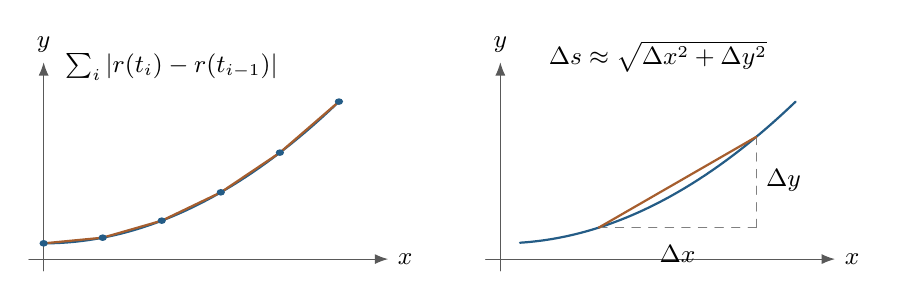
\begin{tikzpicture}[font=\small,>=Latex,line cap=round,line join=round]
\begin{scope}[shift={(0.00000,0.00000)},xscale=1.25,yscale=1]
\draw[->,black!65] (-0.15000,0.00000)--(3.50000,0.00000);
\node[right] at (3.50000,0.00000) {$x$};
\draw[->,black!65] (0.00000,-0.15000)--(0.00000,2.50000);
\node[above] at (0.00000,2.50000) {$y$};
\draw[curveblue,thick] plot[smooth] coordinates {(0.00000,0.20000) (0.02000,0.20008) (0.04000,0.20032) (0.06000,0.20072) (0.08000,0.20128) (0.10000,0.20200) (0.12000,0.20288) (0.14000,0.20392) (0.16000,0.20512) (0.18000,0.20648) (0.20000,0.20800) (0.22000,0.20968) (0.24000,0.21152) (0.26000,0.21352) (0.28000,0.21568) (0.30000,0.21800) (0.32000,0.22048) (0.34000,0.22312) (0.36000,0.22592) (0.38000,0.22888) (0.40000,0.23200) (0.42000,0.23528) (0.44000,0.23872) (0.46000,0.24232) (0.48000,0.24608) (0.50000,0.25000) (0.52000,0.25408) (0.54000,0.25832) (0.56000,0.26272) (0.58000,0.26728) (0.60000,0.27200) (0.62000,0.27688) (0.64000,0.28192) (0.66000,0.28712) (0.68000,0.29248) (0.70000,0.29800) (0.72000,0.30368) (0.74000,0.30952) (0.76000,0.31552) (0.78000,0.32168) (0.80000,0.32800) (0.82000,0.33448) (0.84000,0.34112) (0.86000,0.34792) (0.88000,0.35488) (0.90000,0.36200) (0.92000,0.36928) (0.94000,0.37672) (0.96000,0.38432) (0.98000,0.39208) (1.00000,0.40000) (1.02000,0.40808) (1.04000,0.41632) (1.06000,0.42472) (1.08000,0.43328) (1.10000,0.44200) (1.12000,0.45088) (1.14000,0.45992) (1.16000,0.46912) (1.18000,0.47848) (1.20000,0.48800) (1.22000,0.49768) (1.24000,0.50752) (1.26000,0.51752) (1.28000,0.52768) (1.30000,0.53800) (1.32000,0.54848) (1.34000,0.55912) (1.36000,0.56992) (1.38000,0.58088) (1.40000,0.59200) (1.42000,0.60328) (1.44000,0.61472) (1.46000,0.62632) (1.48000,0.63808) (1.50000,0.65000) (1.52000,0.66208) (1.54000,0.67432) (1.56000,0.68672) (1.58000,0.69928) (1.60000,0.71200) (1.62000,0.72488) (1.64000,0.73792) (1.66000,0.75112) (1.68000,0.76448) (1.70000,0.77800) (1.72000,0.79168) (1.74000,0.80552) (1.76000,0.81952) (1.78000,0.83368) (1.80000,0.84800) (1.82000,0.86248) (1.84000,0.87712) (1.86000,0.89192) (1.88000,0.90688) (1.90000,0.92200) (1.92000,0.93728) (1.94000,0.95272) (1.96000,0.96832) (1.98000,0.98408) (2.00000,1.00000) (2.02000,1.01608) (2.04000,1.03232) (2.06000,1.04872) (2.08000,1.06528) (2.10000,1.08200) (2.12000,1.09888) (2.14000,1.11592) (2.16000,1.13312) (2.18000,1.15048) (2.20000,1.16800) (2.22000,1.18568) (2.24000,1.20352) (2.26000,1.22152) (2.28000,1.23968) (2.30000,1.25800) (2.32000,1.27648) (2.34000,1.29512) (2.36000,1.31392) (2.38000,1.33288) (2.40000,1.35200) (2.42000,1.37128) (2.44000,1.39072) (2.46000,1.41032) (2.48000,1.43008) (2.50000,1.45000) (2.52000,1.47008) (2.54000,1.49032) (2.56000,1.51072) (2.58000,1.53128) (2.60000,1.55200) (2.62000,1.57288) (2.64000,1.59392) (2.66000,1.61512) (2.68000,1.63648) (2.70000,1.65800) (2.72000,1.67968) (2.74000,1.70152) (2.76000,1.72352) (2.78000,1.74568) (2.80000,1.76800) (2.82000,1.79048) (2.84000,1.81312) (2.86000,1.83592) (2.88000,1.85888) (2.90000,1.88200) (2.92000,1.90528) (2.94000,1.92872) (2.96000,1.95232) (2.98000,1.97608) (3.00000,2.00000)};
\draw[accent,thick] (0.00000,0.20000)--(0.60000,0.27200);
\fill[curveblue] (0.00000,0.20000) circle (1.2pt);
\draw[accent,thick] (0.60000,0.27200)--(1.20000,0.48800);
\fill[curveblue] (0.60000,0.27200) circle (1.2pt);
\draw[accent,thick] (1.20000,0.48800)--(1.80000,0.84800);
\fill[curveblue] (1.20000,0.48800) circle (1.2pt);
\draw[accent,thick] (1.80000,0.84800)--(2.40000,1.35200);
\fill[curveblue] (1.80000,0.84800) circle (1.2pt);
\draw[accent,thick] (2.40000,1.35200)--(3.00000,2.00000);
\fill[curveblue] (2.40000,1.35200) circle (1.2pt);
\fill[curveblue] (3.00000,2.00000) circle (1.2pt);
\node[above] at (1.30000,2.15000) {$\sum_i|r(t_i)-r(t_{i-1})|$};
\end{scope}
\begin{scope}[shift={(5.80000,0.00000)},xscale=1.25,yscale=1]
\draw[->,black!65] (-0.15000,0.00000)--(3.40000,0.00000);
\node[right] at (3.40000,0.00000) {$x$};
\draw[->,black!65] (0.00000,-0.15000)--(0.00000,2.50000);
\node[above] at (0.00000,2.50000) {$y$};
\draw[curveblue,thick] plot[smooth] coordinates {(0.20000,0.20800) (0.21867,0.20956) (0.23733,0.21127) (0.25600,0.21311) (0.27467,0.21509) (0.29333,0.21721) (0.31200,0.21947) (0.33067,0.22187) (0.34933,0.22441) (0.36800,0.22708) (0.38667,0.22990) (0.40533,0.23286) (0.42400,0.23596) (0.44267,0.23919) (0.46133,0.24257) (0.48000,0.24608) (0.49867,0.24973) (0.51733,0.25353) (0.53600,0.25746) (0.55467,0.26153) (0.57333,0.26574) (0.59200,0.27009) (0.61067,0.27458) (0.62933,0.27921) (0.64800,0.28398) (0.66667,0.28889) (0.68533,0.29394) (0.70400,0.29912) (0.72267,0.30445) (0.74133,0.30992) (0.76000,0.31552) (0.77867,0.32126) (0.79733,0.32715) (0.81600,0.33317) (0.83467,0.33933) (0.85333,0.34564) (0.87200,0.35208) (0.89067,0.35866) (0.90933,0.36538) (0.92800,0.37224) (0.94667,0.37924) (0.96533,0.38637) (0.98400,0.39365) (1.00267,0.40107) (1.02133,0.40862) (1.04000,0.41632) (1.05867,0.42416) (1.07733,0.43213) (1.09600,0.44024) (1.11467,0.44850) (1.13333,0.45689) (1.15200,0.46542) (1.17067,0.47409) (1.18933,0.48290) (1.20800,0.49185) (1.22667,0.50094) (1.24533,0.51017) (1.26400,0.51954) (1.28267,0.52905) (1.30133,0.53869) (1.32000,0.54848) (1.33867,0.55841) (1.35733,0.56847) (1.37600,0.57868) (1.39467,0.58902) (1.41333,0.59950) (1.43200,0.61012) (1.45067,0.62089) (1.46933,0.63179) (1.48800,0.64283) (1.50667,0.65401) (1.52533,0.66533) (1.54400,0.67679) (1.56267,0.68839) (1.58133,0.70012) (1.60000,0.71200) (1.61867,0.72402) (1.63733,0.73617) (1.65600,0.74847) (1.67467,0.76090) (1.69333,0.77348) (1.71200,0.78619) (1.73067,0.79904) (1.74933,0.81203) (1.76800,0.82516) (1.78667,0.83844) (1.80533,0.85185) (1.82400,0.86540) (1.84267,0.87908) (1.86133,0.89291) (1.88000,0.90688) (1.89867,0.92099) (1.91733,0.93523) (1.93600,0.94962) (1.95467,0.96414) (1.97333,0.97881) (1.99200,0.99361) (2.01067,1.00856) (2.02933,1.02364) (2.04800,1.03886) (2.06667,1.05422) (2.08533,1.06972) (2.10400,1.08536) (2.12267,1.10114) (2.14133,1.11706) (2.16000,1.13312) (2.17867,1.14932) (2.19733,1.16565) (2.21600,1.18213) (2.23467,1.19875) (2.25333,1.21550) (2.27200,1.23240) (2.29067,1.24943) (2.30933,1.26660) (2.32800,1.28392) (2.34667,1.30137) (2.36533,1.31896) (2.38400,1.33669) (2.40267,1.35456) (2.42133,1.37257) (2.44000,1.39072) (2.45867,1.40901) (2.47733,1.42744) (2.49600,1.44600) (2.51467,1.46471) (2.53333,1.48356) (2.55200,1.50254) (2.57067,1.52167) (2.58933,1.54093) (2.60800,1.56033) (2.62667,1.57988) (2.64533,1.59956) (2.66400,1.61938) (2.68267,1.63934) (2.70133,1.65944) (2.72000,1.67968) (2.73867,1.70006) (2.75733,1.72058) (2.77600,1.74124) (2.79467,1.76203) (2.81333,1.78297) (2.83200,1.80404) (2.85067,1.82526) (2.86933,1.84661) (2.88800,1.86811) (2.90667,1.88974) (2.92533,1.91152) (2.94400,1.93343) (2.96267,1.95548) (2.98133,1.97767) (3.00000,2.00000)};
\draw[gray,dashed] (1.00000,0.40000)--(2.60000,0.40000);
\draw[gray,dashed] (2.60000,0.40000)--(2.60000,1.55200);
\draw[accent,thick] (1.00000,0.40000)--(2.60000,1.55200);
\node[below] at (1.80000,0.30000) {$\Delta x$};
\node[right] at (2.60000,1.00000) {$\Delta y$};
\node[above] at (1.60000,2.25000) {$\Delta s\approx\sqrt{\Delta x^2+\Delta y^2}$};
\end{scope}
\end{tikzpicture}
\end{document}
